\documentclass[tikz]{standalone}
% \usetikzlibrary{intersections}
\usetikzlibrary{angles}
\input{../standalonepreamble.tex}

\begin{document}
\tikzset{help lines/.style=very thin}
\tikzset{Karl's grid/.style={help lines,color=blue!50}}

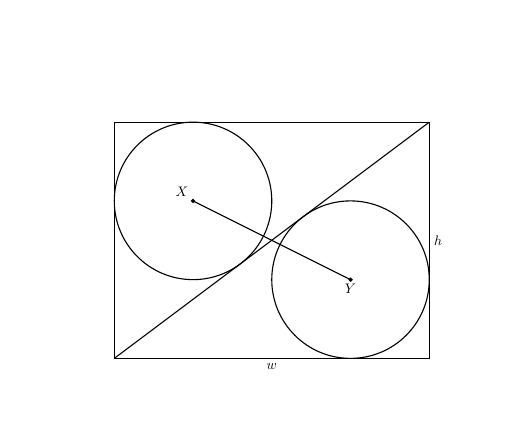
\begin{tikzpicture}[every node/.style={scale=0.5}]
  \clip (-1.1,-0.5) rectangle (4.8,4.2);
  \draw[thin] (0,0) rectangle (4,3);
  \draw (0,0) -- (4,3);
  \draw (1.0, 2.0) circle [radius=1cm];
  \draw (3.0, 1.0) circle [radius=1cm];
  \draw (1.0, 2.0) -- (3.0, 1.0);
  \filldraw (1.0, 2.0) circle [radius=0.2mm];
  \filldraw (3.0, 1.0) circle [radius=0.2mm];
  \draw (1.0,2.0) node[above left] {$X$};
  \draw (3.0,1.0) node[below] {$Y$};
  \draw (2.0,0.0) node[below] {$w$};
  \draw (4.0,1.5) node[right] {$h$};
\end{tikzpicture}

\end{document}
